\section{Graph}


\begin{frame}[fragile]{Graph}
\begin{adjustbox}{max totalsize={.9\textwidth}{.7\textheight},center}
% Define style for nodes
\tikzstyle{every node}=[circle, draw, fill=black!50,
                        inner sep=0pt, minimum width=4pt]
%  Tutte's 8-cage
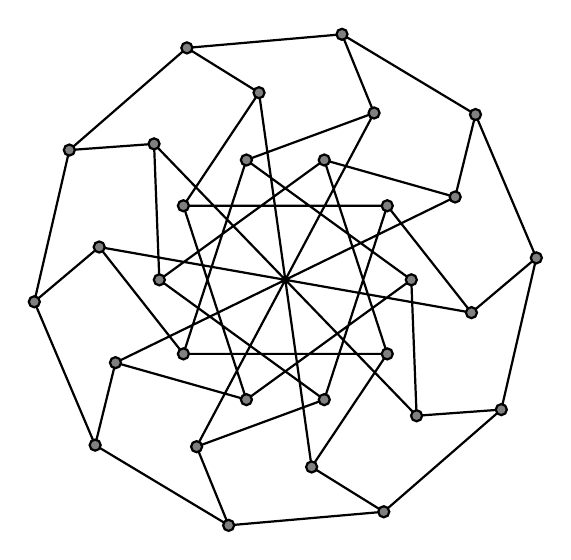
\begin{tikzpicture}[thick,scale=0.8]
    % The following path utilizes several useful tricks and features:
    % 1) The foreach statement is put inside a path, so all the edges
    %    will in fact be a the same path.
    % 2) The node construct is used to draw the nodes. Nodes are special
    %    in the way that they are drawn *after* the path is drawn. This
    %    is very useful in this case because the nodes will be drawn on
    %    top of the path and therefore hide all edge joins.
    % 3) Simple arithmetics can be used when specifying coordinates.
    \draw \foreach \x in {0,36,...,324}
    {
        (\x:2) node {}  -- (\x+108:2)
        (\x-10:3) node {} -- (\x+5:4)
        (\x-10:3) -- (\x+36:2)
        (\x-10:3) --(\x+170:3)
        (\x+5:4) node {} -- (\x+41:4)
    };
\end{tikzpicture}\quad
%
%
% The largest 3-regular graph of diameter 3
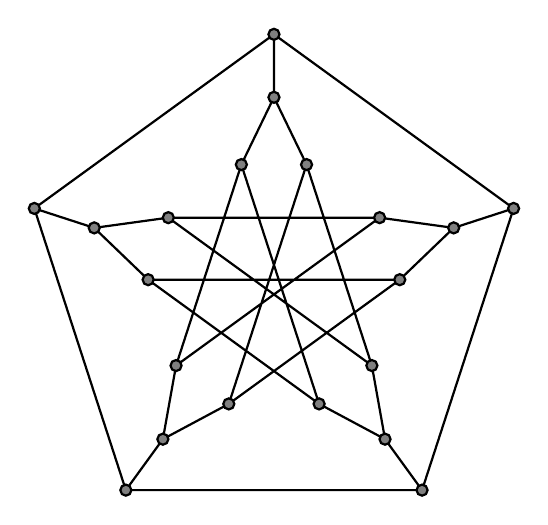
\begin{tikzpicture}[thick,scale=0.8]%
    \draw \foreach \x in {18,90,...,306} {
        (\x:4) node{} -- (\x+72:4)
        (\x:4) -- (\x:3) node{}
        (\x:3) -- (\x+15:2) node{}
        (\x:3) -- (\x-15:2) node{}
        (\x+15:2) -- (\x+144-15:2)
        (\x-15:2) -- (\x+144+15:2)
};
\end{tikzpicture}
\end{adjustbox}
\end{frame}


\begin{frame}[fragile]{Scientific Interactions}
\begin{figure}
\centering
\begin{adjustbox}{max totalsize={.9\textwidth}{.7\textheight},center}
\begin{tikzpicture}[mindmap,
  level 1 concept/.append style={level distance=130,sibling angle=30},
  extra concept/.append style={color=blue!50,text=black}]

  % Applied area: computer science and its subfields

  \begin{scope}[mindmap, concept color=orange, text=white]
    \node [concept] {Informatique}[clockwise from=-5] 
      child {node [concept] (log) {M{\'e}thodes cat{\'e}goriques}}
      child {node [concept] (alg) {Algorithmique}}
      child {node [concept] (cod) {Compression \& transmission}}
      child {node [concept] (img) {Tra{\^i}tement des images}}
      child {node [concept] (opt) {Optimisation}}
      child {node [concept] (res) {R{\'e}seaux}};
  \end{scope}

  % Applied area: theoretical physics and its subfields

  \begin{scope}[mindmap, concept color=red,text=white]
    \node [concept] at (-5,-15) {Physique}
      child [grow=-10, level distance=160]
        {node [concept] (qin) {Calcul quantique}}
      child [grow=20] 
        {node [concept] (csm) {Astronomie \& cosmologie}}
      child [grow=110] 
        {node [concept] (mat) {Mati{\`e}re condens{\'e}e}};
  \end{scope}

  % Applied area: biology and its subfields

  \begin{scope}[mindmap, concept color=green!50!black,text=white]
    \node [concept] at (6.5,-15) {Biologie} 
      child [grow=165, level distance=120] 
        {node [concept] (med) {M{\'e}decine}}
      child [grow=60] 
        {node [concept] (gen) {G{\'e}nomique}};
  \end{scope}

  % Applied area: economics (one subfield)

  \begin{scope}[mindmap, concept color=violet, text=white]
    \node [concept] at (11,-14) {{\'E}conomie}
      child [grow=70, level distance=120] 
        {node [concept] (dec) {Choix \& prise de d{\'e}cision}};
  \end{scope}

  % Researchers listed by their main specialization in mathematics

  \begin{scope}[mindmap, concept color=blue]

    % Combinatorics and discrete mathematics 
    \node [concept, text=white] at (5.2,-10.8) 
      {Combinatoire \& math{\'e}matiques discr{\`e}tes} 
      [clockwise from=150]
      child [concept color=blue!50] {node [concept] (ver) {Vereschagin}}
      child [concept color=blue!50, level distance=125] 
        {node [concept] (kab) {Kabatyanski, Tsfasman, Rybakov, Zykin}}
      child [concept color=blue!50] 
        {node [concept] (kch) {Kucherov, Roytberg}}
      child [concept color=blue!50] {node [concept] (raf) {Raffinot}}
      child [concept color=blue!50, level distance=135]
        {node [concept] (ksh) {Koshevoy}};

    % Partial differential equations
    \node [concept, text=white] at (-3,-11) 
      {Equations aux d{\'e}riv{\'e}es partielles 
        \& m{\'e}thodes num{\'e}riques}
      child [concept color=blue!50, grow=0, level distance=140] 
        {node [concept] (lhc) {Loh{\'e}ac}}
      child [concept color=blue!50, grow=60, level distance=115] 
        {node [concept] (otr) {OTARIE (Sobolevski)}}
      child [concept color=blue!50, grow=95] {node [concept] (ndr) 
        {Nadirashvili}};

    % Probability
    \node [concept, text=white] at (-7.2,-3.2) {Probabilit{\'e}s}
      child [concept color=blue!50, grow=-70, level distance=120] 
        {node [concept] (rbk) {Rybko}};

    % Logic
    \node [concept, text=white] at (11.5,-5) {Logique}
      child [concept color=blue!50, grow=165, level distance=120] 
        {node [concept] (sht) {Shehtman}};
  \end{scope}

  % Connections of researchers to applied subfields

  \begin{pgfonlayer}{background}
    \draw [circle connection bar]
      (kab) edge (cod)
      (kch) edge (alg) edge (gen)
      (lhc) edge (med)
      (ksh) edge (dec)
      (ndr) edge (mat)
      (otr) edge (opt) edge (csm) edge (img)
      (raf) edge (alg) edge (gen)
      (rbk) edge (res) edge (mat)
      (sht) edge (log) edge (dec)
      (ver) edge (qin) edge (cod);
  \end{pgfonlayer}
\end{tikzpicture}
\end{adjustbox}

\caption{Graph Example: Scientific interactions}
\end{figure}
\end{frame}




\begin{frame}[fragile]{Content}
\begin{easylist} \easyitem
& 图的定义
& 图的存储表示
& 图的遍历
\end{easylist}
\end{frame}


\begin{frame}[fragile]{何谓查找表 ?}
\tikz \graph[ layout=VerySimpleDemo, radius=1cm] {
a -- b -- c -- a;
d -- e;
f -- g -- h -- d -- f;
e -- g;
};
\end{frame}


\begin{frame}[fragile]{查找表的分类}
\begin{easylist} \easyitem
& 静态查找表
&& 仅作查询和检索操作的查找表。
& 动态查找表
&& 有时在查询之后,还需要将“查询”结果为“不在查找表中”的数据元素{\em 插入}到查找表中;或者,从查找表中{\em 删除}其“查询”结果为“在查找表中”的数据元素。
\end{easylist}
\end{frame}


\begin{frame}[fragile]{关键字}
\begin{easylist} \easyitem
& 是数据元素(或记录)中某个数据项的值,用以标识(识别)一个数据元素(或记录)。
& 若此关键字可以识别唯一的一个记录,则称之谓“主关键字”。
& 若此关键字能识别若干记录,则称之谓“次关键字”。
\end{easylist}
\end{frame}


\begin{frame}[fragile]{查找}
\begin{easylist} \easyitem
& 根据给定的某个值,在查找表中确定一个其关键字等于给定值的数据元素或(记录)  
& 若查找表中存在这样一个记录,则称“查找成功”:
&& 查找结果:给出整个记录的信息,或指示该记录在查找表中的位置;
& 否则称“查找不成功”,查找结果:
&& 给出“空记录”或“空指针”。
\end{easylist}
\end{frame}


\begin{frame}[fragile]{如何进行查找?}
\begin{easylist} \easyitem
& 查找的方法取决于查找表的结构。
& 由于查找表中的数据元素之间不存在明显的组织规律,因此不便于查找。
& 为了提高查找的效率, 需要在查找表中的元素之间人为地 附加某种确定的关系,换句话说, 用另外一种结构来表示查找表。
\end{easylist}
\end{frame}


\subsection{静态查找表}
\begin{frame}[fragile]{9.1 静态查找表(Static Search Table)}
\begin{easylist} \easyitem

\end{easylist}
\end{frame}


\begin{frame}[fragile]{SSTable}
\begin{lstlisting}[tabsize=8,keywordstyle=\color{red},basicstyle=\small]
public class SSTable {
	List<Element> elements;  //数据元素存放的地方
	int length; //表的长度
}
\end{lstlisting}

\end{frame}


\begin{frame}[fragile]{Element}
\begin{lstlisting}[tabsize=8,keywordstyle=\color{red},basicstyle=\small]
public class Element<K, V> {
	K key;
	V value;
}
\end{lstlisting}
\end{frame}




\begin{frame}[fragile]{}
\begin{easylist} \easyitem

\end{easylist}
\end{frame}


